\documentclass{beamer}

\usepackage{fontspec}
\usepackage{xeCJK}
\setCJKmainfont[BoldFont=Noto Serif CJK TC Bold]{Noto Serif CJK TC}
\XeTeXlinebreaklocale "zh"
\XeTeXlinebreakskip = 0pt plus 1pt
\linespread{1.3}
\allowdisplaybreaks

\usepackage[round]{natbib}
\usepackage{color}
\usepackage{booktabs}
\usepackage{tabularx}
\usepackage{caption}
\usepackage{tikz}
\usepackage{graphicx}
\usepackage{spreadtab}
\usepackage{subfigure}
\usepackage{verbatim}
\usepackage{pgfplotstable}
\usepackage{fancyhdr}
\pgfplotsset{width=12cm}
\pgfplotsset{height=7cm}
\pgfplotsset{compat=1.13}

\usetheme{EastLansing}

\setbeamertemplate{footline}{%
  \hbox{%
    %\begin{beamercolorbox}[wd=.2\paperwidth,ht=3ex,dp=1.75ex,center]{author in head/foot}
      %\insertauthor
    %\end{beamercolorbox}%
    \begin{beamercolorbox}[wd=.9\paperwidth,ht=3ex,dp=1.75ex,left]{section in head/foot}
      $\; \;$ Meta Learning for Low-Resource Speech Recognition
    \end{beamercolorbox}%
    \begin{beamercolorbox}[wd=.1\paperwidth,ht=3ex,dp=1.75ex,center]{number in head/foot}
      \insertframenumber\ /\ \inserttotalframenumber
    \end{beamercolorbox}%
  }
}
\usetikzlibrary{positioning}
\useinnertheme{rectangles}
\usefonttheme{professionalfonts}

\newcommand{\lw}{0.8mm}
\setbeamercovered{transparent}


\title{Meta-Learning for\\ End-to-End Low-Resouce Speech Recognition}
\subtitle{\textcolor[rgb]{0.00,0.50,1.00}{{Speech Processing \& Machine Learning Laboratory}}}
\author{Jui-Yang Hsu}
\date{\today}
\begin{document}

\begin{frame}
\maketitle
\end{frame}

%\begin{frame}{Multilingual Transfer Learning}
  %Find a unified latent space for all languages through shared encoder, \\
  %then use langauge-specific decoder to output token sequence
  %\center 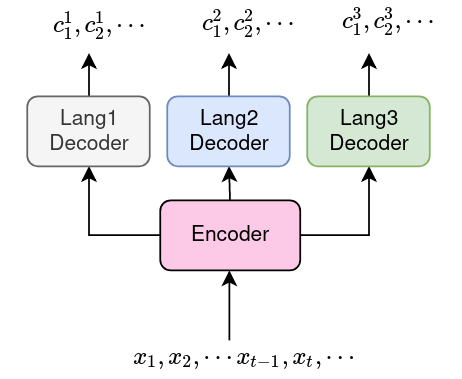
\includegraphics[width=0.5\textwidth]{fig/MultiTaskASR.png}
%\end{frame}


\section{Meta Learning}
\begin{frame}[t]{Meta Learning: Learning to Learn}
  \begin{block}{Goal}
    Fast adaptation on unseen task $D_t$ from a set of pretraining tasks $\{ D_k\}^{K}_{k=1}$ 
  \end{block}

  \pause 

  \begin{itemize}
    \item Assumption: tasks are inherently related (inductive transfer is beneficial)
    \item Definition of task $D_k$: depend on application
  \end{itemize}
\end{frame}

\begin{frame}[t]{What we meta-learn for?}
  \centering Meta-learn \textcolor{blue}{X} to improve learn \textcolor{orange}{Y}
  \pause
  \flushleft \textcolor{blue}{X} (inductive bias) can be
  \begin{itemize}
    \item parameter initialization
    \item optimization strategy (e.g optimizer)
    \item network architecture
    \item distance metric
    \item hyper-parameter
  \end{itemize}
  %$\qquad \cdot$ \\
  %$\qquad \cdot$ \\
  %$\qquad \cdot$
\end{frame}

\begin{frame}[t]{What we meta-learn for?}
  \centering Meta-learn \textcolor{blue}{X} to improve learn \textcolor{orange}{Y}

  \flushleft \textcolor{orange}{Y} (application) can be
  \begin{itemize}
    \item Computer Vision (\citealt{snell2017prototypical}, \citealt{rusu2018meta} ...)
    \item Machine Translation (\citealt{gu2018meta})
    \item Dialogue Generation (\citealt{mi2019meta})
    \item Speaker-Adaptative Training (\citealt{klejch2019speaker})
  \end{itemize}
\end{frame}

\begin{frame}[t]{What we meta-learn for?}
  \centering Meta-learn \textcolor{blue}{parameter initialization} \\ to improve learn \textcolor{orange}{End-to-End Speech Recognition}

  \pause
  \flushleft How to meta-learn \textcolor{blue}{parameter initialization}?
  \begin{itemize}
    \item Model-Agnostic Meta-Learning (MAML) (\citealt{finn2017model})
    \item View different languages' corpus as different tasks
  \end{itemize}

  \pause

  Why \textcolor{orange}{End-to-End Speech Recognition}?
  \begin{itemize}
    \item Voracious for training data
    \item Low-resource 
  \end{itemize}
\end{frame}


\begin{frame}[t]{Recap: Multilingual Transfer Learning}

  \begin{enumerate}
    \item Pretraining (Multilingual Training): \\ learn good \textbf{initialization for adaptation} on pretraining langauges
    \item Adaptation: \\ use the learned initialization to adapt on target language
  \end{enumerate}
\end{frame}

\begin{frame}[t]{Recap: Multilingual Transfer Learning}
  We apply MAML in Pretraining stage to
  \begin{itemize}
    \item improve overall performance (CER)
    \item reduce over-fitting on pretraining langauges
  \end{itemize}
\end{frame}


\begin{frame}[t]{Quick Overview of MAML}
  \begin{block}{Goal}
    Learn initialization parameters $\theta^\star$, such that performing few gradient steps during meta-test time (adaptation) can minimize loss on $D_t$
  \end{block}

\end{frame}

\begin{frame}[t]{Quick Overview of MAML}
  \begin{block}{Meta-objective}
    \begin{equation*}
    \theta^\star = \arg \min_\theta \frac{1}{K}\sum_{k=1}^{K}\mathcal{L}_{D_k^{test}}(\theta - \alpha \nabla \mathcal{L}_{D_k^{tr}}(\theta))
    \end{equation*}
  \end{block}

  \begin{itemize}
    \item $\mathcal{L}_D$: Loss calculated on $D$
    \item $D_k^{tr}$, $D_k^{test}$ are disjoint sets of $D_k$
    %\item Use SGD with $D_k^{tr}$
  \end{itemize}
\end{frame}

\begin{frame}[t]{Quick Overview of MAML}
  \begin{block}{Meta-objective}
    \begin{equation*}
    \theta^\star = \arg \min_\theta \frac{1}{K}\sum_{k=1}^{K}\mathcal{L}_{D_k^{test}}(\theta - \alpha \nabla \mathcal{L}_{D_k^{tr}}(\theta))
    \end{equation*}
  \end{block}

  \begin{itemize}
    \item Use SGD with $D_k^{tr}$ as update rule (can be more steps)
    \item Used SGD with independently-sampled $D_k^{test}$ to update the parameters
  \end{itemize}

  \vspace{1em}

  Intuition: MAML explicitly optimized the loss of the \textbf{adapted} parameters
\end{frame}

\begin{frame}
	\begin{center}
    \LARGE{Proposed Approach}
	\end{center}
\end{frame}

\section{Proposed Approach}
\begin{frame}[t]{Model Architecture}
  \center 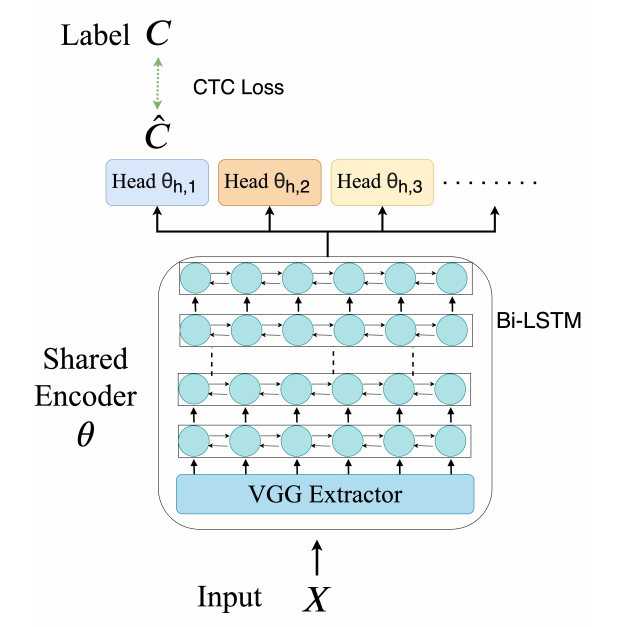
\includegraphics[width=0.55\textwidth]{fig/model_arch.png}
\end{frame}

\begin{frame}[t]{Illustration of 1 meta episode in MetaASR}
  Step (Meta Episode) 1 (Collect gradient)
  \center 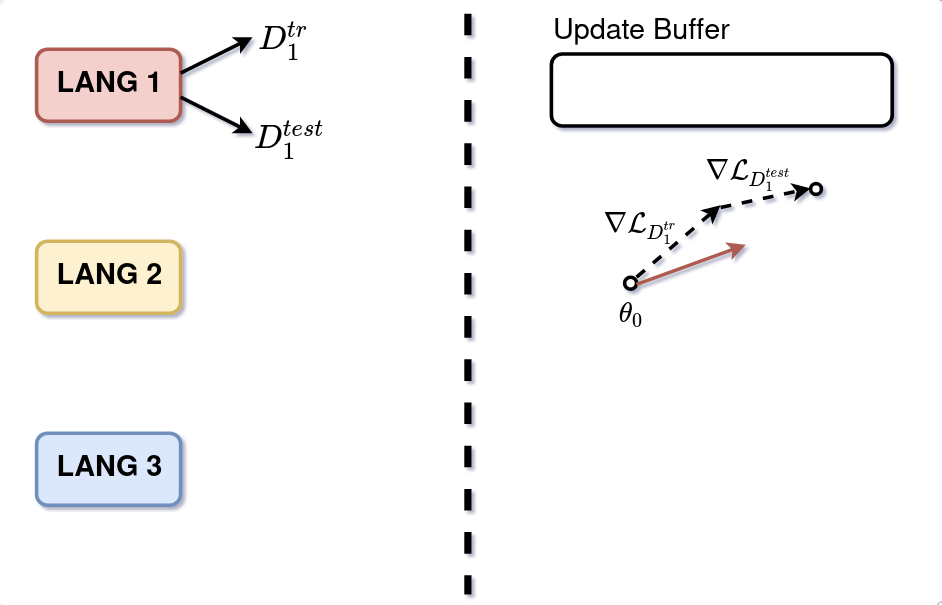
\includegraphics[width=0.85\textwidth]{fig/meta_step1.png}
  %\only<1-2> \center 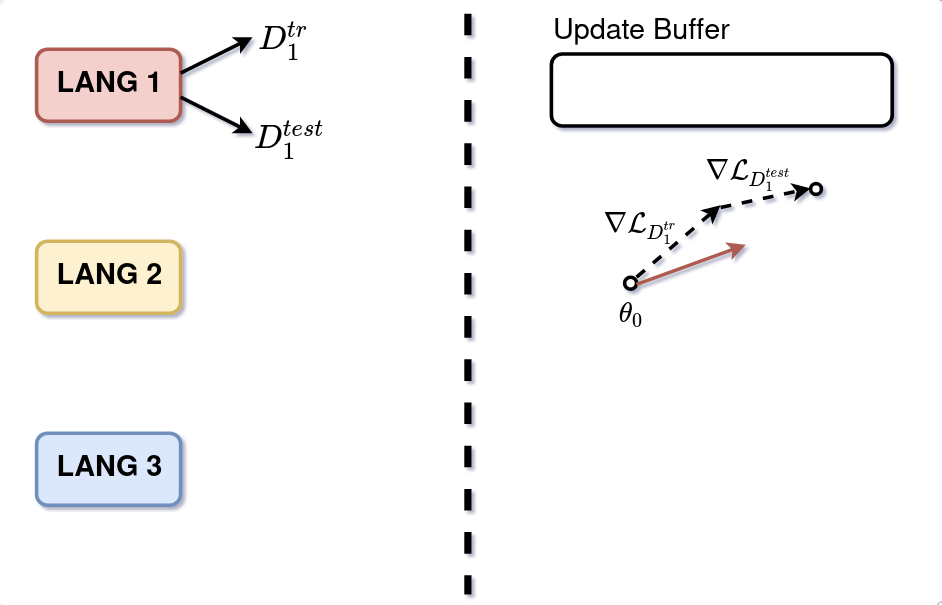
\includegraphics[width=0.85\textwidth]{fig/meta_step1.png}
  %\only<2-3> \center 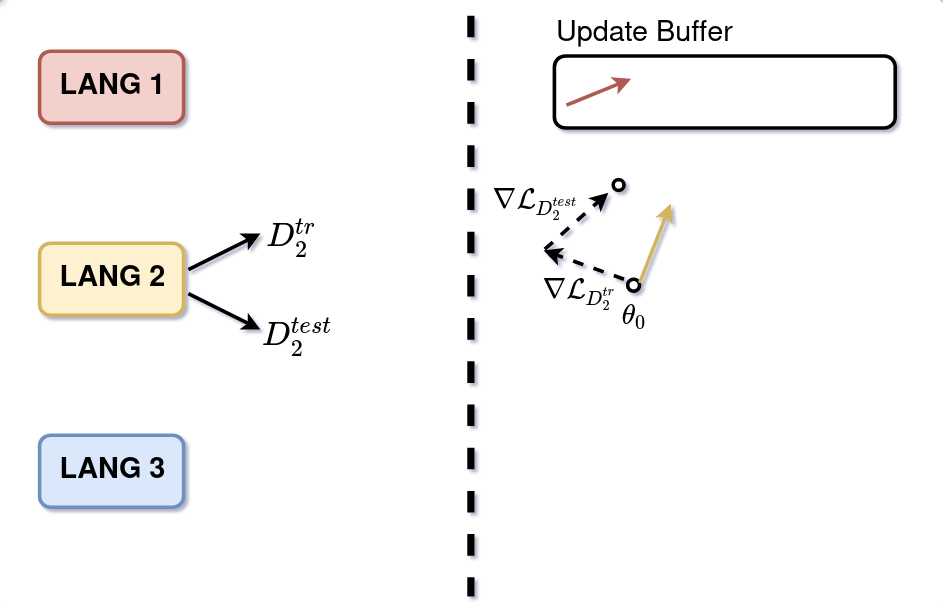
\includegraphics[width=0.85\textwidth]{fig/meta_step2.png}
  %\only<3> \center 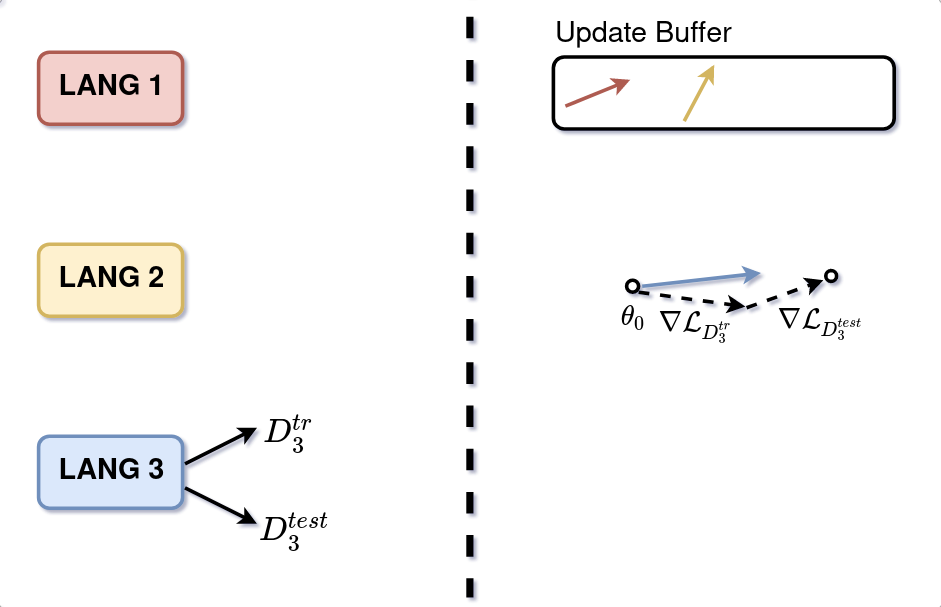
\includegraphics[width=0.85\textwidth]{fig/meta_step3.png}
\end{frame}

\begin{frame}[t]{Illustration of 1 meta episode in MetaASR}
  Step (Meta Episode) 1 (Collect gradient)
  \center 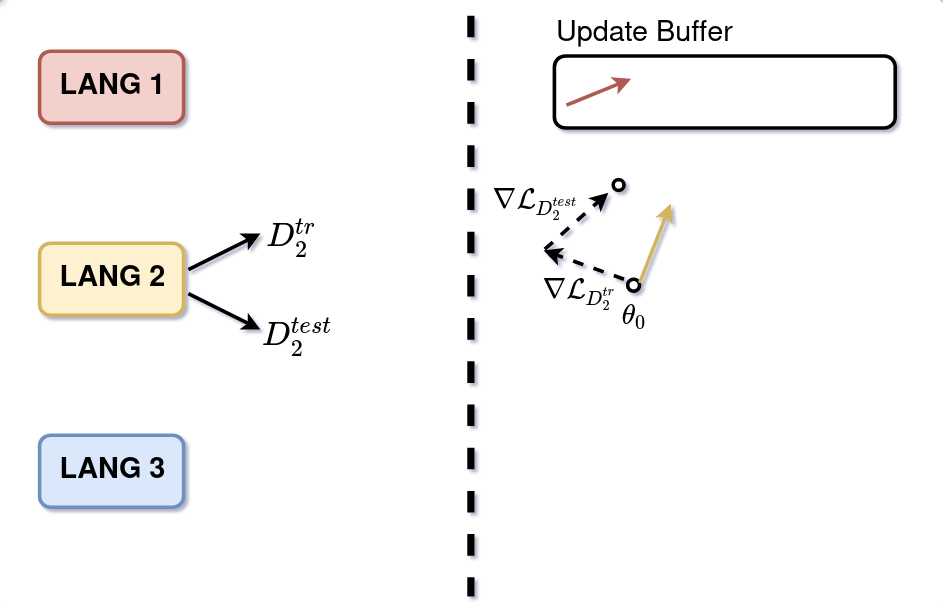
\includegraphics[width=0.85\textwidth]{fig/meta_step2.png}
\end{frame}

\begin{frame}[t]{Illustration of 1 meta episode in MetaASR}
  Step (Meta Episode) 1 (Collect gradient)
  \center 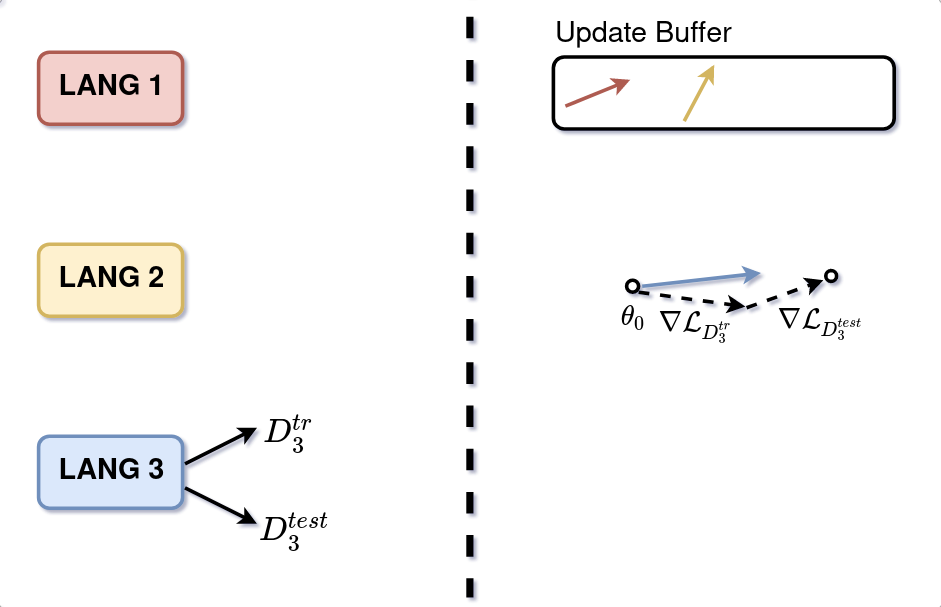
\includegraphics[width=0.85\textwidth]{fig/meta_step3.png}
\end{frame}

\begin{frame}[t]{Illustration of 1 meta episode in MetaASR}
  Step (Meta Episode) 1 (Collect gradient finished)
  \center 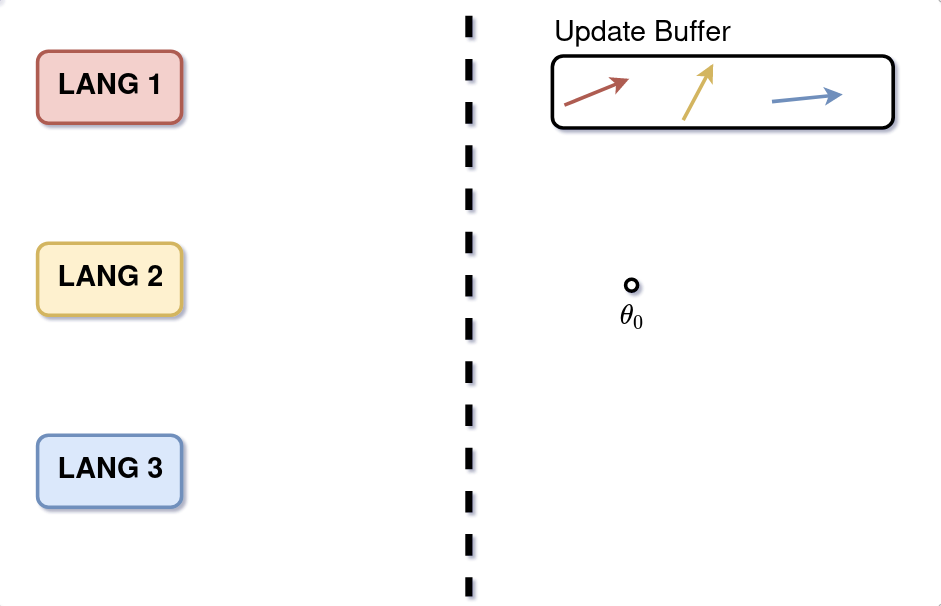
\includegraphics[width=0.85\textwidth]{fig/meta_before_update.png}
\end{frame}

\begin{frame}[t]{Illustration of 1 meta episode in MetaASR}
  Step (Meta Episode) 1 \textcolor{red}{Update}
  \center 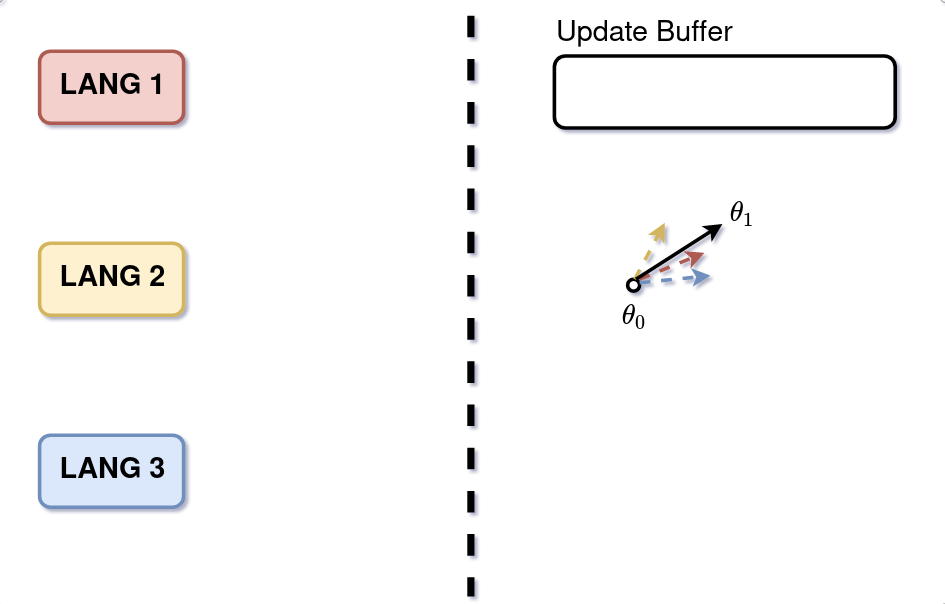
\includegraphics[width=0.85\textwidth]{fig/meta_update.png}
\end{frame}

\begin{frame}
	\begin{center}
    \LARGE{In contrast to Multitask Training}
	\end{center}
\end{frame}

\begin{frame}[t]{Baseline: Multitask Training (MultiASR)}
  Multitask training (MultiASR) acts as main backbone in multilingual pretraining
  \vspace{2em}
  \begin{enumerate}
    \item Random draw one sample in one pretraining langauge \\ (either uniform sampling or $\propto$ corpus size)
    \item Update through SGD on that sample
  \end{enumerate}
\end{frame}

\begin{frame}[t]{Baseline: Multitask Training (MultiASR)}
  Step 1 
  \center 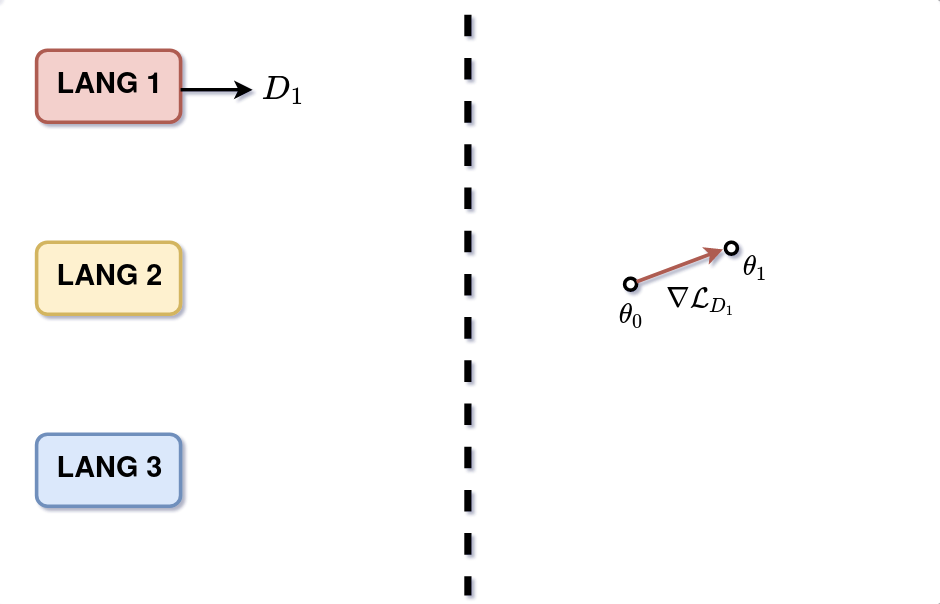
\includegraphics[width=0.85\textwidth]{fig/multi_step1.png}
\end{frame}

\begin{frame}[t]{Baseline: Multitask Training (MultiASR)}
  Step 2 
  \center 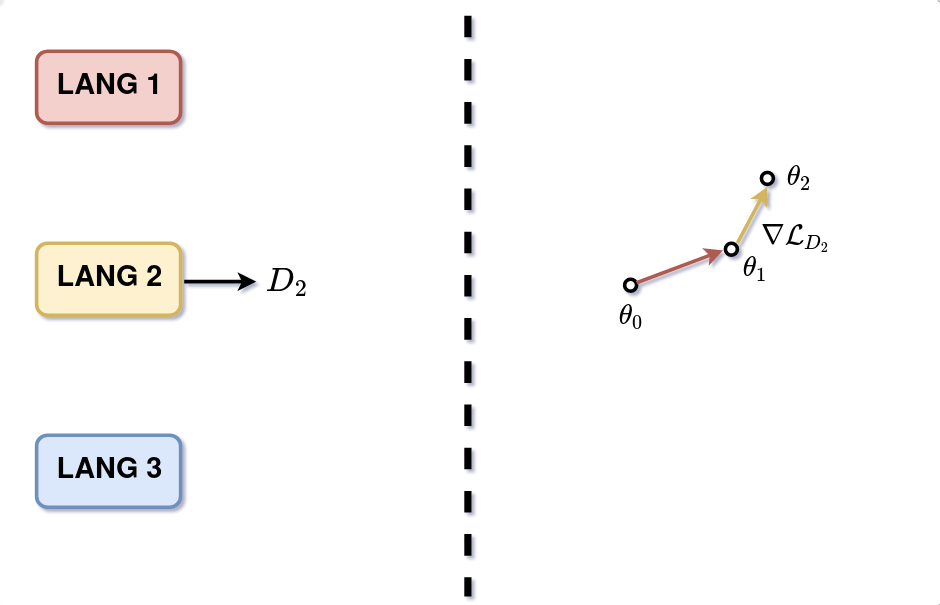
\includegraphics[width=0.85\textwidth]{fig/multi_step2.png}
\end{frame}

\begin{frame}[t]{Baseline: Multitask Training (MultiASR)}
  Step 3 
  \center 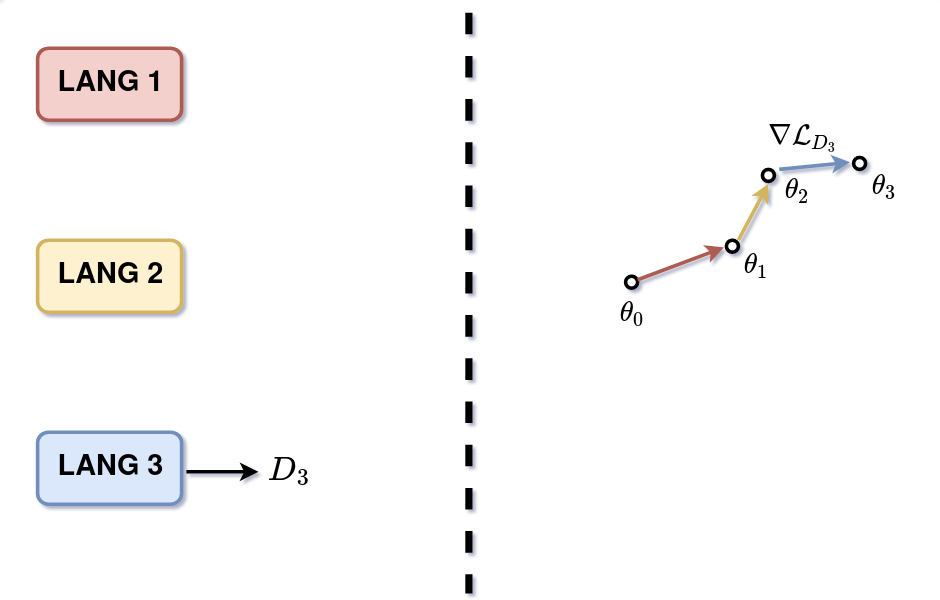
\includegraphics[width=0.85\textwidth]{fig/multi_step3.png}
\end{frame}

\section{Experimental Results}
\begin{frame}[t]{Questions we care about}
  \begin{enumerate}
    \item Is adaptation performance of MetaASR better than MultiASR ?
    \item Is MetaASR avoid over-fitting on pretraining languages (unlike MultiASR)?
    \item If MultiASR equipped with uniform sampling strategy (like MetaASR), is 2 still true?
  \end{enumerate}
\end{frame}

\begin{frame}[t]{Experimental Setting}
  Corpus: IARPA-BABEL (Conversational Telephone Speech)
  \begin{itemize}
    \item FLP: 40 $\sim$ 80 hr
    \item LLP: 10hr (subset of FLP)
  \end{itemize}
  \pause
  Languages:
  \begin{itemize}
    \item Source: Bengali (Bn), Tagalog (Tl), Zulu (Zu), Turkish (Tr), Lithuanian (Lt), Guarani (Gn)
    \item Target: Vietnamese (Vi), Swahili (Sw), Tamil (Ta), Kurmanji (Ku)
    \item Validation: Cross-validation
  \end{itemize}
\end{frame}

\begin{frame}[t]{CER on FLP}
  Refer to Question 1
  \center 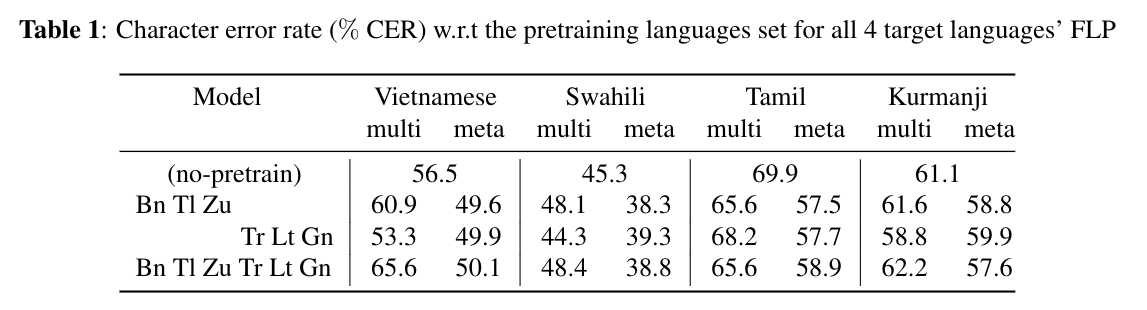
\includegraphics[width=1.0\textwidth]{fig/flp_table.png}

  \begin{itemize}
    \item Adaptation from MetaASR performs better than random initialization
    \item Fix pretraining languages and target language, MetaASR is always better than MultiASR
  \end{itemize}
\end{frame}

%\begin{frame}[t]{Learning Curve}
  %Refer to Question 2 \& 3
  %\center 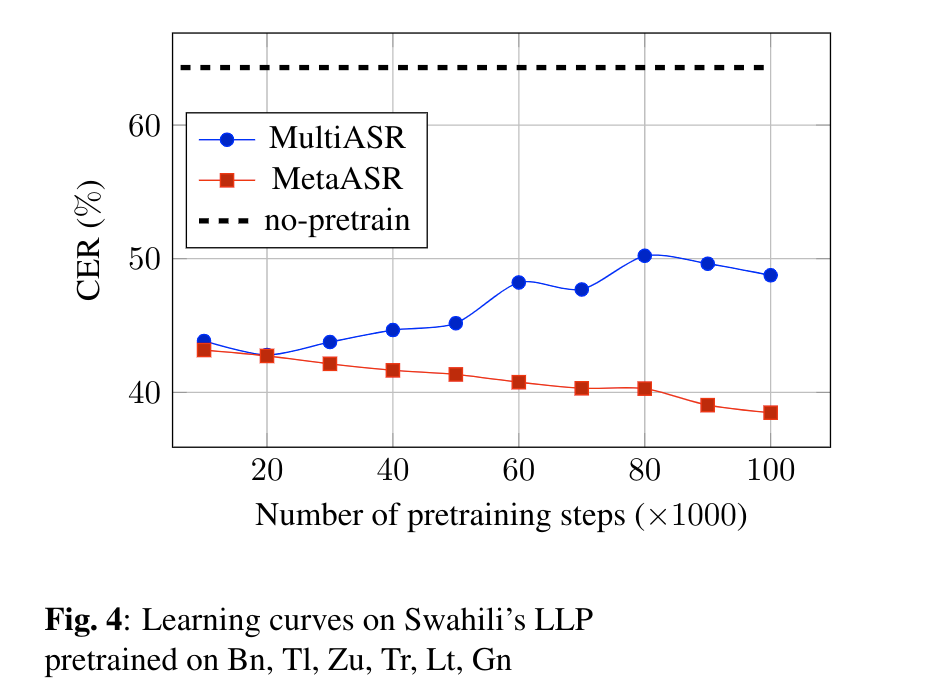
\includegraphics[width=0.7\textwidth]{fig/lr.png}
%\end{frame}

%\begin{frame}[t]{Conclusion}
  %Meta-learned initialization
  %\begin{itemize}
    %\item overall performance is better than multitask-learned one
    %\item doesn't overfit so easily
  %\end{itemize}
  %\pause
  %\vspace{3em}
  %\center new research direction for speech community
%\end{frame}

\begin{frame}[t]{Learning Curve (dev cer on LLP)}
  Pretraining Languages: Bn, Tl, Zu; Target Language: Vi

    \begin{figure}[H]
    \centering
    %\hspace{-5.2cm}
    \begin{tikzpicture}[trim axis left, trim axis right]

    \begin{axis}[
      width=1.0\linewidth,
      height=0.5\linewidth,
      legend entries={MetaASR, MultiASR, MultiASR (uniform), no-pretrain},
      legend style={cells={anchor=west}, at={(0.3,-0.1)}, font=\tiny},
      xlabel = {Pretraining steps ($\times 10^3$)},
          xmin=0,
          xmax=100,
          grid=both,
          ylabel={CER}]
    \addplot+[smooth]table{stat/107-near3/fomaml-107-devcer};
    \addplot+[smooth]table{stat/107-near3/multi-107-devcer};
    \addplot+[smooth]table{stat/107-near3/reptile-107-devcer};
    \addplot[style=ultra thick,dashed,] coordinates {(0,58.9) (100,58.9)};
    \end{axis}
    \end{tikzpicture}
  \end{figure}
\end{frame}

\begin{frame}[t]{Learning Curve (dev cer on LLP)}
  Pretraining Languages: Bn, Tl, Zu; Target Language: Sw

    \begin{figure}[H]
    \centering
    %\hspace{-5.2cm}
    \begin{tikzpicture}[trim axis left, trim axis right]

    \begin{axis}[
      width=1.0\linewidth,
      height=0.5\linewidth,
      legend entries={MetaASR, MultiASR, MultiASR (uniform), no-pretrain},
      legend style={cells={anchor=west}, at={(0.3,-0.1)}, font=\tiny},
      xlabel = {Pretraining steps ($\times 10^3$)},
          xmin=0,
          xmax=100,
          grid=both,
          ylabel={CER}]
    \addplot+[smooth]table{stat/107-near3/fomaml-202-devcer};
    \addplot+[smooth]table{stat/107-near3/multi-202-devcer};
    \addplot+[smooth]table{stat/107-near3/reptile-202-devcer};
    \addplot[style=ultra thick,dashed,] coordinates {(0,42.1) (100,42.1)};
    \end{axis}
    \end{tikzpicture}
  \end{figure}
\end{frame}

\begin{frame}[t]{Conclusion}
  \begin{itemize}
    \item Adaptation using meta-learned parameter is beneficial
    \item Can be applied to different applications beyond ASR
    \item Need more analysis of the performance gain
  \end{itemize}
\end{frame}

\begin{frame}
	\begin{center}
    \LARGE{Discussion}
	\end{center}
\end{frame}

\bibliographystyle{plainnat}
\bibliography{M335}

\end{document} 
